\chapter{Introduction}
\label{chap:introduction}

%\todo{soll hier ein kurzer überblick über die Arbeit und das Kapitel gegeben werden? Also wo was beschrieben ist usw?}



%\section{Importance of Research and Motivation}
Traffic congestion in urban areas became a bigger problem every year in the past decades. Increasing traffic causes several issues, for example high monetary and environmental costs by using gasoline and by emitting $CO_2$ to the environment. There are several strategies to reduce urban traffic to mitigate these problems like for example new investments in public transport infrastructure. However, the usage of private cars in cities won't stop in the next decades, but increase. According to a study by Hao et al. \cite{HAO2016121} car sales will continue to grow in the upcoming decades and therefore also traffic will continue to become worse in big cities. Thus, it is important to find ways to reduce traffic in urban areas.

With more vehicles driving in urban areas, there also comes the need for a sufficient number of parking spaces. Finding parking spaces in urban areas can be a really difficult, frustrating and time consuming task for drivers. There often exists some information about the availability of parking spaces in parking garages, but in most cities the situation of road side parking is rather non-transparent. This not only leads to frustrated drivers, who are searching for parking spaces a long time, but again contributes to urban traffic congestion as many cars have to drive around close to their destination while searching for free parking spaces. 

There are many studies, which show that the searching for parking spaces adds a lot of traffic. In 2013 a study by Nawaz et al. \cite{Nawaz:2013:PSB:2500423.2500438} showed that about 30\% of traffic congestion is created by drivers looking for free parking spaces. Another study \cite{TexasMobilityReport} found that alone in 2007 searching for parking spaces caused costs of about 78 billion US dollars by using 2.9 billion gallons of wasted gasoline and 4.2 billion lost hours only in the United States. Furthermore, this obviously causes a lot of $CO_2$ emissions which is not only bad for the environment and contributes to climate change, but also lowers the quality of living in big cities through the significant amount of air pollution.

One of the most important contributors to high search times for parking spaces is not only the lack of vacant parking spaces, but also the lack of information, if and where free parking spaces are available. Therefore, one way to mitigate many of the above stated problems is to determine the current parking space situation in the city and make it accessible to the public (e.g. via web application), so that drivers can efficiently navigate to a vacant parking space, or even decide if they want to go by car or use public transportation, depending on the number of parking spaces available close to their destination. 

However, detection of road side parking spaces and their states is a challenging task. Of course an obvious approach to the problem would be to put stationary sensors to every parking space in the city, which check, if the corresponding parking space is occupied or vacant. This, however, has the drawback to be very expensive as, for big cities, thousands of sensors would have to be bought, installed and maintained. Furthermore, because the state of parking parking spaces does not often change, the high frequency of sensing with such a system would be rather inefficient.





\section{Drive-By park sensing}

A promising novel approach to sense a city's parking situation is the use of mobile sensors instead of static ones. Crowd sensing has the advantage to be usually more cost effective and can provide sufficient accuracy for the purpose of providing parking space availability maps.

There are several approaches to mobile parking availability sensing, which will be discussed in chapter \ref{chap:relatedwork}. This thesis will focus on "drive-by park sensing". The idea of drive-by sensing approaches is that there are sensing vehicles which are driving through the city and collecting data of their environment through mounted sensors. Using the collected data parking cars and vacant parking spaces should be detected. There already exists a prototype implementation of such a system. In 2013, Mathur et al. \cite{Mathur:2010:PDS:1814433.1814448} presented their system, called ParkNet, which continuously measured the distance to the nearest obstacle on the right side of the road, as well as the location of the sensing vehicle through a GPS sensor. Using these data, they used thresholding to detect parking cars and vacant parking spaces. A more detailed description of their work is being described in section \ref{related_driveby_park_sensing_distance}.

Figure \ref{fig:driveby_standard_parking_situation} shows a standard drive-by scenario of a sensing vehicle which passes two parallel parked cars and a vacant parking space in between them. The distance measurements while passing the parked cars will be much shorter than the measurements taken while passing the vacant parking space. This should allow a basic algorithm to recognize parking cars and vacant parking spaces.

\begin{figure}
	\centering
	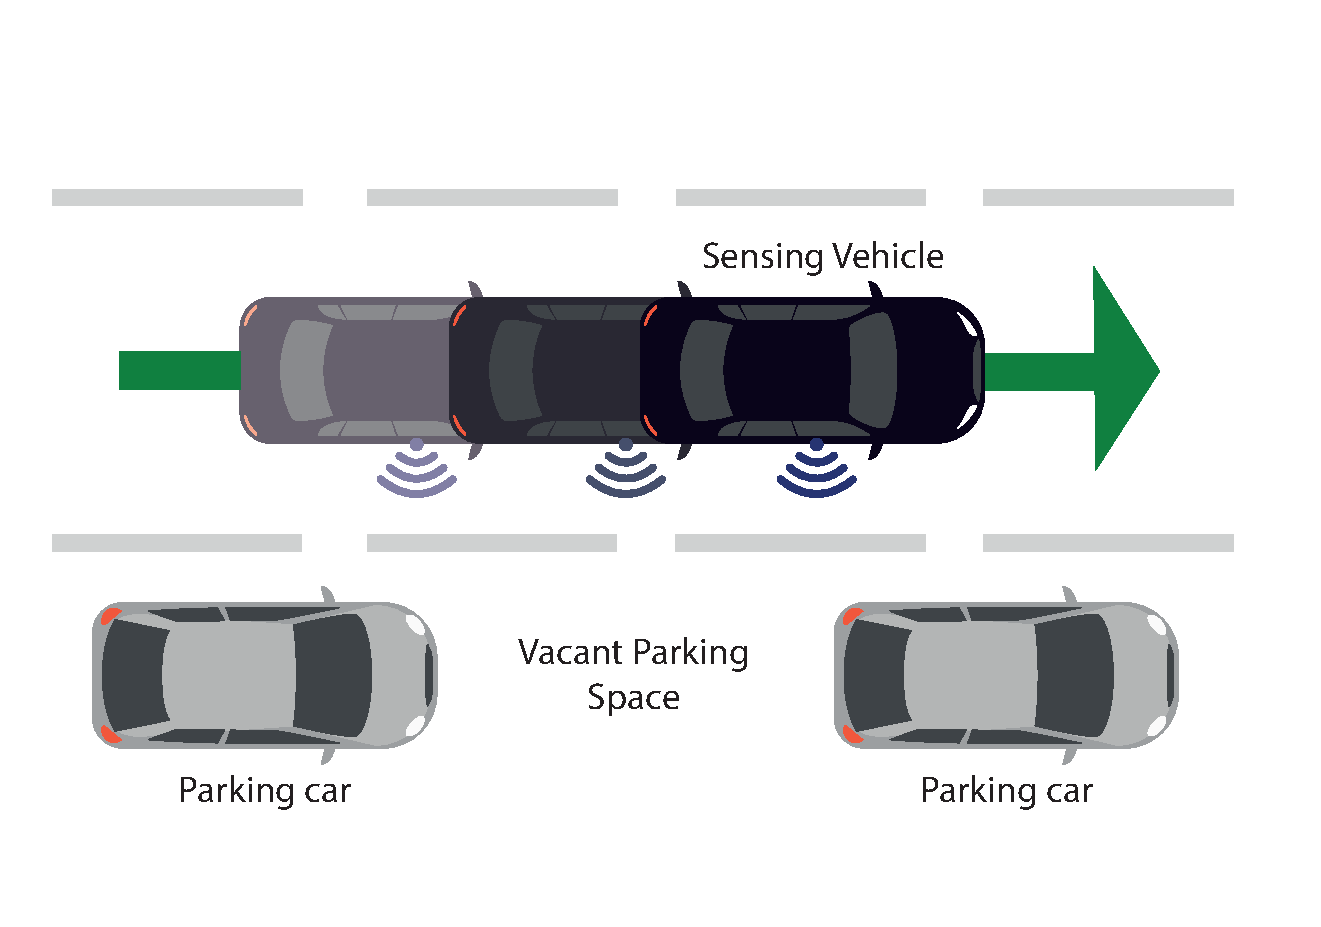
\includegraphics[width=0.9\textwidth]{img/drive-by-parking-situation-pictogram.eps}
	\caption{The sensing vehicle passes two parked cars and should identify a vacant spot in between using distance and location measurements. \todo{Hier Referenz zu Parknet-Paper??? Ähnliche Grafik...}}
	\label{fig:driveby_standard_parking_situation}
\end{figure}

However, the situation which is shown in figure \ref{fig:driveby_standard_parking_situation} is an idealistic one. In real life traffic, there will be much more complex situations to face, which are not as easily detectable and which might influence the success of the detection. For instance, the sensing vehicle might not drive in the right-most lane, therefore the measured distances will be much longer. Another possible issue are other driving cars, motorcycles or bicycles which the sensing car overtakes. There are many of such distractions which have to be filtered out to ensure that there are as few false detections as possible. 
The existing ParkNet prototype does not take any of such situations into account, because it was only evaluated on parallel parking cars on single lane roads.

The high complexity of urban traffic and the many distractions during sensing make it nearly impossible to create a rule set based on the sensor measurements which would be able to detect parking situations at a sufficient accuracy. Therefore, simple thresholding as applied in the ParkNet prototype will not work in real life traffic scenarios. Furthermore, such rule sets would have to be created for each city individually because of the different nature of the roads and the parking spaces. For instance, the distance between roads and parking spaces can vary highly in two different cities. Thus, to be able to detect parking situations, new methods have to be found, which should be more flexible to distractions and changes in the environment.

%There are several approaches to mobile parking availability sensing, which will be discussed in chapter \ref{chap:relatedwork}. In this thesis a "drive-by park sensing" approach will be implemented, tested and evaluated. The approach works as follows: Several sensing vehicles drive through the city and measure their environment using two sensors. The first sensor measures the distance to the nearest obstacle on the right side of the road (often a parking car). A LIDAR (Light Detection and Ranging) sensor is being used to measure the distance, because of its high range and high measuring frequency. The second sensor is a GPS sensor which tracks the position of the vehicles. So while the vehicles are driving through the city, both sensors are constantly recording their environment. Using these data parking cars should be detected and vacant parking spaces should be derived using parking space maps.

%Figure \ref{fig:driveby_standard_parking_situation} shows a standard scenario of a sensing vehicle which passes two parallel parked cars and a vacant parking space in between them. The distance measurements while passing the parked cars will be much shorter than the measurements taken while passing the vacant parking space. This should allow a basic algorithm to recognize parking cars and vacant parking spaces.

%\begin{figure}
%	\centering
%	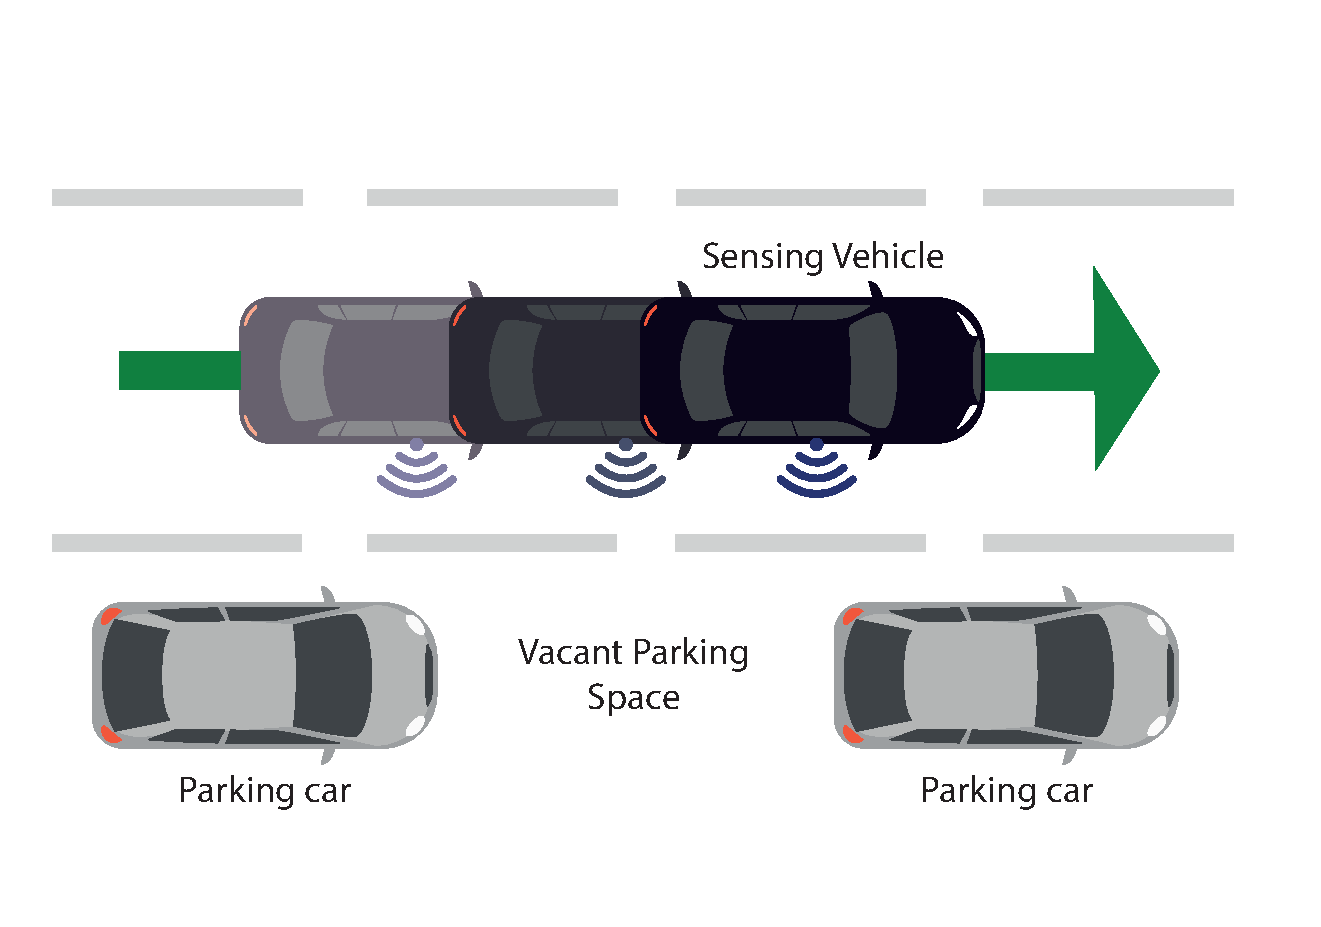
\includegraphics[width=0.9\textwidth]{img/drive-by-parking-situation-pictogram.eps}
%	\caption{The sensing vehicle passes two parked cars and should identify a vacant spot in between using distance and location measurements. \todo{Hier Referenz zu Parknet-Paper??? Ähnliche Grafik...}}
%	\label{fig:driveby_standard_parking_situation}
%\end{figure}

%However, the situation which is shown in figure \ref{fig:driveby_standard_parking_situation} is an idealistic one. In real life traffic, there will be much more complex situations to face, which are not as easily detectable and which might influence the success of the detection. For instance, the sensing vehicle might not drive in the right-most lane, therefore the measured distances will be much longer. Another possible issue are other driving cars, motorcycles or bicycles which the sensing car overtakes. There are many of such distractions which have to be filtered out to ensure that there are as few false detections as possible. 

%The high complexity of urban traffic and the many distractions during sensing make it nearly impossible to create a rule set based on the sensor measurements which would be able to detect parking situations at a sufficient accuracy. Furthermore, such rule sets would have to be created for each city individually because of the different nature of the roads and the parking spaces. For instance, the distance between roads and parking spaces can vary highly between two cities. In this thesis several machine learning techniques are being tested and compared to each other to find out if machine learning can be used to identify complex road side parking situations, to filter out distractions like overtaking situations and to detect vacant parking spaces. 

%During test runs with a prototype car in Linz, Austria, sample measurements are being recorded, where the focus lies on creating very diverse and realistic situations. The recorded data is being filtered and pre-processed before it is used as input for the machine learning algorithms. 






\section{Research goals and methodology}

The overall goal of this thesis is to determine which accuracy can be achieved for detecting the parking space situation in urban real world traffic scenarios using drive-by park sensing. Furthermore, distracting situations should be identified and strategies to cope with them should be found to be able to keep the detection accuracy high. In contrast to existing approaches in this thesis machine learning will be applied to classify different road traffic and parking scenarios to be able to better cope with the high variety of situations possible. As a first step, sensor data has to be collected in real world traffic scenarios including distance sensor measurements and GPS locations of the sensing vehicle. To be able to apply supervised learning all sensor measurements have to get assigned their ground truth manually. As next step different machine learning algorithms will be applied, evaluated and compared to each other in terms of accuracy for the different classes. The detailed methodology which will be followed includes the following steps:

\begin{description}

\item[Building a test bed] As a first step a test bed has to be built, which is able to access the required sensors to record all the necessary data. A Raspberry Pi will be used as processing device because of its popularity and the many compatible sensors which work with this platform. It is connected to a LIDAR-Lite v3 sensor which continuously measures the distance to the nearest obstacle on the right side of the road. A GPS receiver will track the location of the sensing vehicle and a camera will be used to record images of the ground truth for evaluation purposes only. In section \ref{sec:system_design} the complete setup of the test bed is described as well as all the specific hard ware parts and their abilities.

\item[Acquiring a dataset] As soon as the test bed is ready, the sensors should be mounted on the prototype car to be able to start recording the dataset. Test drives should be done in some selected streets in Linz, Austria with the focus of variety of the recorded situations. The test scenes should include single lane as well as multi lane streets and measurements in all streets should be done several times. Furthermore, the car should be driving as it would in regular traffic (not only in the right most lane, etc...) and the scenes should also include high and low traffic scenarios to have a high amount of diverse data. All measured distances, GPS locations and ground truth images have to be saved to files with the according timestamps to be able to evaluate the results of different approaches later on. Furthermore, using the images taken by the camera, ground truth values will be manually labelled in different classes (Parked car, free space, overtaken car, ...). A detailed description about the dataset and the ground truth tagging can be found in section \todo{ref} \ref{sec:dataset}.

\item[Data processing and segmentation] As next step the measured sensor values have to be preprocessed and filtered in order for the following algorithms to work. Sensing and overflow errors as well as outliers in the measurements should be identified and removed before further processing. After the raw data has been filtered, the sensor data has to be segmented. As parking cars and other cases which should be classified consist of several sensor measurements, the corresponding sensor measurements should be grouped together and merged to segments which will be later classified. All preprocessing steps and the segmentation process are described in more detail in section \todo{ref} \ref{sec:data_processing}.

\item[Classification using basic machine learning techniques] Features on the created segments are calculated (for instance length, average distance and variation of the distances) and are being used to train and evaluate several machine learning algorithms which will be compared on their performance. Furthermore, some deep learning models will also be evaluated on the raw sensor data of the segments and will be compared to common machine learning results. The results of all experiments can be found in section \todo{ref} \ref{sec:ml_results}.

\item[Further improvements] \todo{todo}

\end{description}






%\section{Detailed Approach and Goals}
%The overall aim of this thesis is to evaluate if it is possible to reach a sufficient high accuracy in road side parking detection on multi lane roads using a sensing vehicle which drives through the city and senses parking spaces while driving by. 
%For the parking detection an optical distance sensor will be used to measure the distance to the nearest obstacle on the right side of the road (in many cases a parking car). This sensor will be mounted on the co-driver's side of the car and will continuously measure the distance while the car is driving. Furthermore, a GPS sensor will be used to include the spatial information of the vehicle. Using these measurements, the prototype should support accurate detection of free parking spaces in challenging road situations. Potential challenges for road-side parking detection are: 
%\begin{itemize}
%\item multi-lane detection
%\item handling inaccuracies in GPS measurements
%\item differentiation of free parking spaces and other free spaces
%\item varying vehicle speed
%\item differentiation between perpendicular/parallel parking spaces
%\end{itemize}
%
%%In a first step, the sensor will be tested on accuracy and reliability. 
%In a first step, after the sensors have been mounted on a car, test measurements will be collected while driving through some selected streets in Linz, Austria. The test scenes should include single lane- as well as multi lane streets and measurements in all streets should be done several times. To determine the ground truth of the parking availability a camera will be used, which takes pictures of the parking situation at the street during the tests.
%
%%After these measurements have been taken, first an algorithm should be developed which only works for single lane streets. The algorithm should be evaluated on the test measurements and the result of the evaluation are parking space count accuracy and parking occupancy rate accuracy. This can later be used as baseline in comparison to multi lane road detection. 
%
%After these measurements have been taken, the measurements should be analyzed, pre-processed, and then an algorithm should be developed (or learned) to classify the current parking situation. An important part of the algorithm will be the handling of multi lane roads, because there are many special cases which have to be considered. First of all, the lane in which the sensing vehicle is going has to be detected and has to be incorporated in the algorithm. Furthermore, the system should also detect when the car overtakes another driving car, because this could lead to falsely detected parking spaces.
%
%In a final step, possible approaches should be evaluated, which can further enhance the results. For example, the cooperation of multiple sensing vehicles which are going at the same time at the same street can maybe help to increase the parking detection accuracy. Finally, the results of single- and multi lane detection should be evaluated and compared in terms of parking space count accuracy and parking occupancy rate accuracy. 
%Furthermore, the lane detection algorithm based on the distance sensor will be evaluated on its performance.











%This section contains some things you will often use in a thesis.
%
%In the following a paper found in literature.bib is cited \cite{empe:2002th}.
%
%Use TIKZ to draw a graph as shown in figure \ref{fig:splits}.
%
%\begin{figure}
%\centering
%\begin{subfigure}[b]{0.5\textwidth}
%	\centering
%	\begin{tikzpicture}[scale=.5,auto=left,every node/.style={draw,circle}]
%		\node (n8) at (-2,8) {8};
%		\node (n7) at (0,6)  {7};
%		\node (n6) at (0,10) {6};
%		\node (n4) at (5,8)  {4};
%		\node (n5) at (8,10) {5};
%		\node (n1) at (11,8) {1};
%		\node (n2) at (8,6)  {2};
% 		\node (n3) at (2,8)  {3};
%
%		\foreach \from/\to in {n6/n3,n4/n5,n5/n1,n1/n2,n2/n5,n2/n4,n3/n4,n8/n6,n8/n7,n8/n3,n7/n3}
%	    	\draw (\from) -- (\to);
%		\draw [dotted, ultra thick] (6.5,11) -- (6.5,5);
%	\end{tikzpicture}
%	\caption{Non-optimal Split}
%\end{subfigure}
%\begin{subfigure}[b]{0.5\textwidth}
%	\centering
%	\begin{tikzpicture}[scale=.5,auto=left,every node/.style={draw,circle}]
%		\node (n8) at (-2,8) {8};
%		\node (n7) at (0,6)  {7};
%		\node (n6) at (0,10) {6};
%		\node (n4) at (5,8)  {4};
%		\node (n5) at (8,10) {5};
%		\node (n1) at (11,8) {1};
%		\node (n2) at (8,6)  {2};
% 		\node (n3) at (2,8)  {3};
%
%		\foreach \from/\to in {n6/n3,n4/n5,n5/n1,n1/n2,n2/n5,n2/n4,n3/n4,n8/n6,n8/n7,n8/n3,n7/n3}
%	    	\draw (\from) -- (\to);
%		\draw [dotted, ultra thick] (3.5,11) -- (3.5,5);
%	\end{tikzpicture}
%	\caption{Optimal Split}
%\end{subfigure}
%\caption{Splits in Structural Graph Partitioning}
%\label{fig:splits}
%\end{figure}
%
%\begin{itemize}
%	\item This is an item
%	\item And this is another one
%\end{itemize}
%
%Include a PDF as a picture. How about this CAB (Compute Aggregate Broadcast) diagram shown in figure \ref{img:arch}.
%
%\cpic{imgs/dgms/bsp-basic.pdf}{Compute Aggregate Broadcast computing paradigm}{img:arch} 
%
%How about another picture with a state machine \ref{fig:globalpregelstate}?
%
%\begin{figure}
%\centering
%	\begin{tikzpicture}[->,>=stealth,scale=.4,auto=left,every node/.style={}]
%		\tikzset{state/.style={draw,ellipse}}
%		\tikzset{start/.style={}}
%		\tikzset{textlabel/.style={}}
%
%		\node [start] (start) at (0, 12) {started} ;
%		\node [state] (init) at (0, 9)  {init} ;
%		\node [state] (processing) at (0, 6)  {processing} ;
%		\node [state] (messaging) at (0, 3) {messaging} ;
%		\node [state] (global) at (10, 4.5) {global} ;
%		\node [start] (end) at (0, 0) {terminated} ;
%
%		\path (start) edge (init);
%		\path (init) edge (processing);
%		\path (processing) edge (messaging);
%		\path (messaging) edge (end);
%		\path (messaging) edge [bend right] (global);
%		\path (global) edge [bend right] (processing);
%
%		\node [textlabel] (continue) at (7, 1) {\emph{activeVertices > 0}};
%		\node [textlabel] (halt) at (-5, 1) {\emph{activeVertices = 0}};
%	\end{tikzpicture}
%\caption{Global State Machine}
%\label{fig:globalpregelstate}
%\end{figure}
%
%Or include some Java code.
%
%\lstinputlisting[caption={HelloWorld}, language=Java, firstline=3, lastline=9, label=lst:pagerank]{code/HelloWorld.java}
